Auf eine  Ausf\"uhrliche Fehlerrechnung  wurde in  Absprache mit  dem Dozenten
verzichtet, die  Messtoleranzen des  experimentellen Aufbaus und  der Ger\"ate
wurden daher auch nicht erfasst.

Aus den unterschiedlichen Werten  der Leitf\"ahigkeiten k\"onnen aber trotzdem
Mittelwerte, Fehler und Standardabweichungen bestimmt werden.

Dazu  wurden die  g\"angigen Formeln  benutzt; Tabelle~\ref{tab:errorAnalysis}
enth\"ahlt eine Auflistung der Resultate. Es wurden s\"amtliche gemachten Fits
ber\"ucksichtigt  (also N\"aherungen  und exakte  L\"osungen), bie  Berechnung
erfolgte in  einem Python-Script, das  seine Werte  aus den Scripts  f\"ur die
Fits erh\"ahlt. Somit  ist sichergestellt,  dass zur Berechnung  auch wirklich
die Werte  verwendet werden, mit  welchen die Plots erstellt  worden sind. Der
\LaTeX-Code f\"ur die Ergebnisse wurde  ebenfalls aus diesem Script generiert,
wie auch bei den Listings f\"ur die Fits.

\begin{align*}
    \text{Mittelwert:~}             \overline{x} & = \frac{1}{N} \sum_{i=1}^{N}{x_i} \\
    \text{absoluter Fehler:~}   s_{\overline{x}} & = \sqrt{ \frac{\sum_{1}^{N}{(x_i-\overline{x})^2}}{N \cdot (N-1)}} \\
    \text{relativer Fehler:~}   r                & = \frac{s_{\overline{x}}}{\overline{x}} \\
    \text{Standardabweichung:~} s_{\overline{x}} & = \sqrt{ \frac{\sum_{1}^{N}{(x_i-\overline{x})^2}}{N-1}} \\
\end{align*}


{%
    \begin{center}
    \captionof{table}{%
        Mittelwerte, Fehler und Standardabweichung f\"ur die Leitf\"ahigkeiten
    }
    \label{tab:errorAnalysis}
    \sisetup{%
        %math-rm=\mathtt,
        scientific-notation=engineering,
        table-format = +3.4e+2,
        round-precision = 4,
        round-mode = figures,
    }
    \begin{tabular}{lr}
    \toprule
        $\overline{\sigma}_{Alu}    $ & $\SI{21031250.0}{\ampere\per\volt\per\meter}$ \\
        $s_{\overline{\sigma}_{Alu}}$ & $\SI{856224.181049733}{\ampere\per\volt\per\meter}$ \\
        $r_{\overline{\sigma}_{Alu}}$ & $\num{0.0407119967215326}$ \\
        $sdev_{\overline{\sigma}_{Alu}}$ & $\SI{2421767.69854466}{\ampere\per\volt\per\meter}$ \\
        $\overline{\sigma}_{Cu}     $ & $\SI{52800000.0}{\ampere\per\volt\per\meter}$ \\
        $s_{\overline{\sigma}_{Cu}} $ & $\SI{200006.624890277}{\ampere\per\volt\per\meter}$ \\
        $r_{\overline{\sigma}_{Cu}} $ & $\num{0.00378800425928555}$ \\
        $sdev_{\overline{\sigma}_{Cu}} $ & $\SI{447228.409204961}{\ampere\per\volt\per\meter}$ \\
        $\overline{\sigma}_{St}     $ & $\SI{1190000.0}{\ampere\per\volt\per\meter}$ \\
        $s_{\overline{\sigma}_{St}} $ & $\SI{28108.0504482257}{\ampere\per\volt\per\meter}$ \\
        $r_{\overline{\sigma}_{St}} $ & $\num{0.0236202104606939}$ \\
        $sdev_{\overline{\sigma}_{St}} $ & $\SI{62851.5115172261}{\ampere\per\volt\per\meter}$ \\

    \bottomrule
    \end{tabular}
    \end{center}
}


Man   k\"onnte    jetzt   nat\"urlich    noch   evaluieren,    inwiefern   die
Ber\"ucksichtigung der Werte  aus den N\"aherungen und  den exakten L\"osungen
gerechtfertigt  ist,  oder  ob  allenfalls  nur  die  Werte  aus  den  exakten
L\"osungen  zu ber\"ucksichtigen  w\"aren,  oder ob  beide  jeweils mit  einer
Gewichtung  ber\"ucksichtigt  werden   sollten.

Aus  Zeitgr\"unden  wird  hier  auf diese  Ausf\"uhrungen  verzichtet. Es  sei
jedoch  angemerkt,  dass keine  der  N\"aherungen  extrem dramatisch  von  den
Werten  der exakten  L\"osungen  abweicht. Wollte man  wirklich penibel  sein,
w\"are  in  den Augen  des  Autors  sowieso eine  ``richtige''  Fehlerrechnung
mit  Ber\"ucksichtigung der  Unsicherheiten  in  Ger\"aten und  Versuchsaufbau
durchzuf\"uhren.

Schlussendlich  ist   nicht  das  Erlangen  exaktest-m\"oglicher   Zahlen  das
prim\"are Ziel  dieses Versuches,  sondern die Demonstration  des Skineffektes
und die experimentelle Best\"atigung, dass Leitwerte f\"ur Materialien aus der
Literatur nicht als absolut gegeben  betrachtet werden sollten, oder zumindest
ist dies die  Ansicht des Autors. Beides ist in seinen  Augen gut demonstriert
worden.

%
\begin{equation}
    \sigma_{Cu}
        = \overline{\sigma}_{Cu} \pm s_{\overline{\sigma}_{Cu}}
        = \SI[separate-uncertainty = true]{52.8 \pm 0.2 }{\ampere\per\volt\per\meter}
       % = \SI[separate-uncertainty = true]{52800000.0 \pm 200006.624890277 }{\ampere\per\volt\per\meter}
\end{equation}

%
\begin{equation}
    \sigma_{St}
        = \overline{\sigma}_{St} \pm s_{\overline{\sigma}_{St}}
        = \SI[separate-uncertainty = true]{1.19 \pm 0.03 }{\ampere\per\volt\per\meter}
        %= \SI[separate-uncertainty = true]{1190000.0 \pm 28108.0504482257 }{\ampere\per\volt\per\meter}
\end{equation}

%
\begin{equation}
    \sigma_{Alu}
        = \overline{\sigma}_{Alu} \pm s_{\overline{\sigma}_{Alu}}
        = \SI[separate-uncertainty = true]{21.0 \pm 0.9 }{\mega\ampere\per\volt\per\meter}
        %= \SI[separate-uncertainty = true]{21031250.0 \pm 856224.181049733 }{\ampere\per\volt\per\meter}
\end{equation}


%
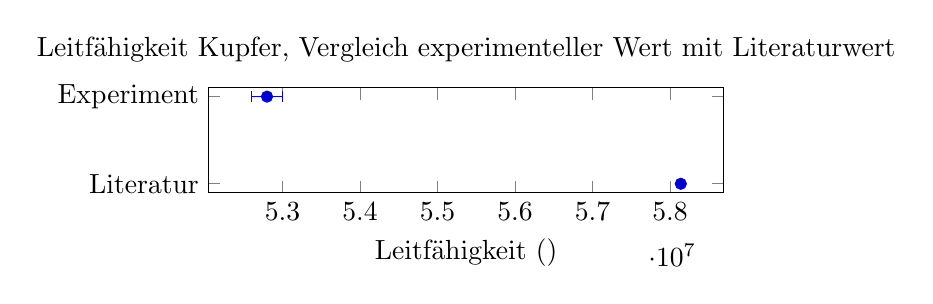
\begin{tikzpicture}
    \begin{axis}[
        try min ticks=2,
        width=.67\textwidth,
        height=.24\textwidth,
        title = {Leitf\"ahigkeit Kupfer, Vergleich experimenteller Wert mit Literaturwert},
        xlabel = {Leitf\"ahigkeit ($\si{\ampere\per\volt\per\meter}$)},
        symbolic y coords = {Literatur,Experiment}
    ]
    \addplot+[
        only marks,error bars/.cd,
        x dir=both,x explicit,
        error bar style={line width=0.5pt},
        ]
    coordinates {%
        (58139534.883720934,Literatur)
        (52800000.0,Experiment) +- (200006.624890277,0)
    };
    \end{axis}
\end{tikzpicture}
\captionof{figure}{%
    Vergleich  der  experimentell   bestimmten  Leitf\"ahigkeit  f\"ur  Kupfer
    mit  dem   Literaturwert  aus   Kuchlings  \emph{Taschebuch   der  Physik}
    \cite{ref:kuchling:resistivityTable}%
    }

%
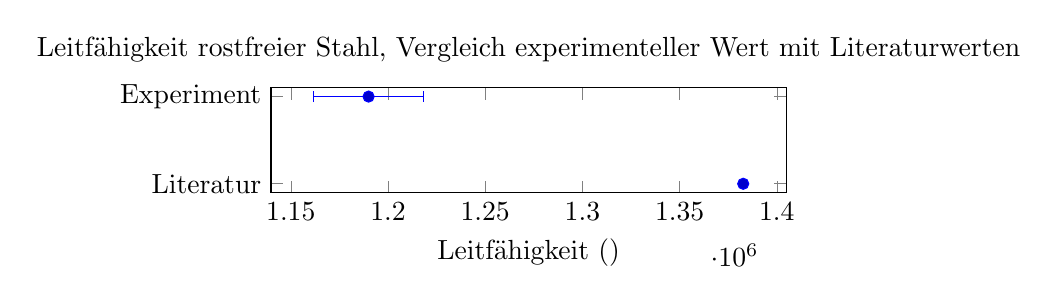
\begin{tikzpicture}
    \begin{axis}[
        try min ticks=2,
        width=.67\textwidth,
        height=.24\textwidth,
        title = {Leitf\"ahigkeit rostfreier Stahl, Vergleich experimenteller Wert mit Literaturwerten},
        xlabel = {Leitf\"ahigkeit ($\si{\ampere\per\volt\per\meter}$)},
        symbolic y coords = {Literatur,Experiment}
    ]
    \addplot+[
        only marks,error bars/.cd,
        x dir=both,x explicit,
        error bar style={line width=0.5pt},
        ]
    coordinates {%
        (1382711.1306243965,Literatur)
        (1190000.0,Experiment) +- (28108.0504482257,0)
    };
    \end{axis}
\end{tikzpicture}
\captionof{figure}{%
    Vergleich  der experimentell  bestimmten Leitf\"ahigkeit  f\"ur rostfreien
    Stahl  mit  einem  aus   Literaturwerten  bestimmten  Wert  (siehe  Anhang
    \ref{app:steel})%
    }

%
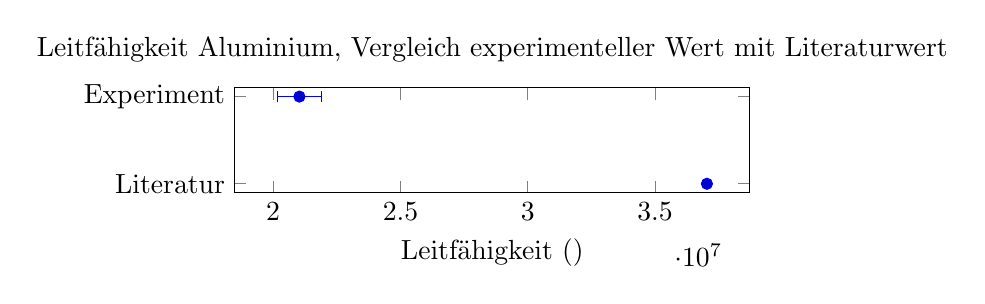
\begin{tikzpicture}
    \begin{axis}[
        try min ticks=2,
        width=.67\textwidth,
        height=.24\textwidth,
        title = {Leitf\"ahigkeit Aluminium, Vergleich experimenteller Wert mit Literaturwert},
        xlabel = {Leitf\"ahigkeit ($\si{\ampere\per\volt\per\meter}$)},
        symbolic y coords = {Literatur,Experiment}
    ]
    \addplot+[
        only marks,error bars/.cd,
        x dir=both,x explicit,
        error bar style={line width=0.5pt},
        ]
    coordinates {%
        (37037037.03703704,Literatur)
        (21031250.0,Experiment) +- (856224.181049733,0)
    };
    \end{axis}
\end{tikzpicture}
\captionof{figure}{%
    Vergleich  der experimentell  bestimmten  Leitf\"ahigkeit f\"ur  Aluminium
    mit  dem   Literaturwert  aus   Kuchlings  \emph{Taschebuch   der  Physik}
    \cite{ref:kuchling:resistivityTable}%
    }

